\chapter{Individual CONStraints: specifics of the implementation}
\label{chapter10}
\setcounter{enums}{0}


This chapter dives into the details of implementing ICONS (Individual
CONStraints)\is{Individual CONStraints} into MRS (Minimal Recursion
Semantics (\citealt{copestake:etal:05}),\is{MRS} or Meaning
Representation System in the current context) by constraining lexical
types and phrasal types. Section \ref{10:sec:lexical} shows how information
structure is dealt with in various lexical types.
Section \ref{10:sec:monoclausal} gives an explanation of information structure
constraints on phrasal types. Next, Section \ref{9:sec:other-constraints}
presents three additional constraints for configuring information
structure in a specific way.  Building upon the hierarchies and
constraints presented thus far, Section \ref{9:sec:samples} illustrates how
information structure is represented via \isi{ICONS} in four languages
(\ili{English}, \ili{Japanese}, \ili{Korean}, and \ili{Russian}).


\section{Lexical types}
\label{10:sec:lexical}


This section largely addresses which lexical item inherits from which
\tdl{icons-lex-item} type out of \tdl{no-icons-lex-item},
\tdl{basic-icons-lex-item}, \tdl{one-icons-lex-item}, and
\tdl{two-icons-lex-item}. They are constrained as presented in the
following AVMs.


\myexe{\enumsentence{\label{avm:icons-lex-item}
\begin{tabular}[t]{lllll}
\evnup{a.} & \evnup{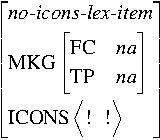
\includegraphics{pdf/no-icons-lex-item.pdf}} & & \evnup{b.} &
\evnup{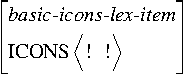
\includegraphics{pdf/basic-icons-lex-item.pdf}} \\ \evnup{c.} &
\evnup{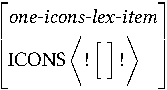
\includegraphics{pdf/one-icons-lex-item.pdf}} & & \evnup{d.} &
\evnup{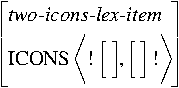
\includegraphics{pdf/two-icons-lex-item.pdf}} \\
\end{tabular}}}


\noindent The first two AVMs do not inherently have an \tdl{info-str}
element on the \isi{ICONS} list,\is{\textit{info-str}} but
information-structure related rules can insert a value into the list
for the second type.  That is, if there is a clue for identifying its
information structure value, a value of \tdl{info-str} is introduced
into the list of \isi{ICONS} and its TARGET is co-indexed with the
HOOK{$\mid$}INDEX of the word.  The last two inherently have non-empty
\isi{ICONS} lists. That means that they lexically have an
\tdl{info-str} value in ICONS.\is{\textit{info-str}}



Lexical entries that cannot be marked with respect to information
structure inherit from \tdl{no-icons-lex-item}
(\ref{avm:icons-lex-item}a). In other words, information structure
markings are not-applicable to them, a constraint formalized as [MKG
  [FC \tdl{na}, TP \tdl{na}]].\is{MKG}\is{relative pronoun} For
example, relative pronouns and expletives in \ili{English} are
instances of \tdl{no-icons-lex-item}.  Other contentful items
introducing an EP inherit from one of the types in
(\ref{avm:icons-lex-item}b--d). The choice among them depends on how
many clauses are subcategorized by the lexical type.  The prefixes
represent how many clauses are created by the type: \tdl{Basic-} means
the lexical type does not include any clausal subject or clausal
complement in ARG-ST. \tdl{One-} means either a clausal subject or a
clausal complement is subordinate to the lexical type. \tdl{Two-}
means there exists a clausal subject and also a clausal complement.
If a verbal type forms a monoclausal construction, the
\tdl{icons-lex-item} type of that verbal item is the basic one
(i.e.\ \tdl{basic-icons-lex-item}).  If a verbal type has ARG-ST
information that includes one or more clausal argument(s)
(i.e.\ multiclausal), its \tdl{icons-lex-item} type is either
\tdl{one-icons-lex-item} (a sentential complement or a sentential
subject) or \tdl{two-icons-lex-item} (both of them).  The extra
\tdl{info-str} values in (\ref{avm:icons-lex-item}c--d) are required
for this purpose.



\subsection{Nominal items}
\label{10:ssec:nominal}

Nominal items, including common nouns, proper nouns, and pronouns,
inherit from \tdl{basic-icons-lex-item}.  One exceptional lexical type
is that of expletives (e.g.\ \textit{it} in \ili{English}), because
they cannot be marked with respect to information structure
\citep{lambrecht:96}.  Expletives inherit from
\tdl{no-icons-lex-item}.  One question regarding \tdl{info-str} of
nominal items is whether different types of nominals can participate
in information structure in the same way and with the same status. The
current work does not recognize any difference in the information
structure of nominal items.  In other words, other than
\tdl{basic-icons-lex-item}, there is no further information structure
constraint on nominal items.


Pronouns have been regarded as a component associated with information
structure in a different way \citep{lambrecht:96}.  Pronouns, roughly
speaking, can be divided into two categories, such as (i) unaccented
and (ii) accented. \citeauthor{lambrecht:96} argues that the
distinction between these two categories can be sufficiently explained
in terms of information structure.  Across languages, (i) unaccented
pronouns preferentially involve topics.  This finding is bolstered by
the evidence that unaccented pronouns are the most frequently used
form of expressing \isi{topic} in Spoken \ili{French}
\citep{lambrecht:86}.  Besides, unaccented pronouns cannot be used for
expressing \isi{focus}, because they are incompatible with
\myref{def:buring:10:ch10-1}.\is{focus prominence}

\myexe{\enumsentence{\label{def:buring:10:ch10-1} Focus Prominence:
    Focus needs to be maximally
    prominent. \citep[277]{buring:10}}}

\noindent On the other hand, (ii) accented pronouns can be divided
again into (ii-a) those with a \isi{topic}-marking accent, and (ii-b)
those with a focus-marking accent. \citeauthor{lambrecht:96}
illustrates the linguistic distinction between (ii-a) and (ii-b) in
Italian as follows.

\myexe{\eenumsentence{\label{exe:lambrecht:pro:ita}
\item\shortex{2}
{\textsc{Io} & \textsc{pago}.}
{I & pay.}
{`\textsc{I}'ll pay.' [ita]}
\item\shortex{2}
{Pago & \textsc{io}.}
{pay & I}
{`\textsc{I}'ll pay.' [ita] \citep[115]{lambrecht:96}}}}


\noindent The preverbal pronoun \textit{\textsc{Io}} in
(\ref{exe:lambrecht:pro:ita}a) expresses a \isi{topic}, with a rising
intonation contour. On the other hand, the pronoun conveying a
\isi{focus} meaning in (\ref{exe:lambrecht:pro:ita}b) occurs
sentence-finally, and has a falling intonation contour, indicating the
end of the assertion.


From a theoretical point of view, it seems clear that pronouns show
different behaviors in packaging information.\footnote{The nominal
  items also differ from each other in discourse status.
  \citet{kaiser:09} argues that the use of different kinds of
  referring expressions is relevant to the salience of the
  antecedents; the more salient antecedent it refers to, the more
  reduced a form (e.g.  dropped subjects) appears.  That is, selecting
  a type of referential form largely hinges on how salient the
  antecedent is.  The discourse status of nominal categories that take
  \tdl{ref-ind} (a subtype of \tdl{individual}) as the value type of
  HOOK{$\mid$}INDEX is represented as COG-ST (COGnitive-STatus) in the
  current \lingo \isi{Grammar Matrix} system \citep{bender:goss:08}.
  Discourse status is related to information status (e.g.\ given
  \vs. new); COG-ST covers information status from a higher
  level. Information status, as discussed in Chapter~\ref{chapter3},
  has often been studied in tandem with information structure, but it
  is neither a necessary nor a sufficient condition for information
  structure.  In sum, since discourse status is not directly
  responsible for representing information structure, the current work
  leaves discourse-related information to future work.} However, the
current work, based on text processing, cannot deploy such a
division. Phenomena related to (ii) can be modeled with hypothetical
suffixes such as \textit{-a} and \textit{-b}, however the responsibility is borne by
the hypothetical suffixes or alternatively lexical rules introducing
the prosodic information, not the pronouns themselves.





\subsection{Verbal items}
\label{10:ssec:verbal}


The analysis proposed here uses the event variable associated with the
head of the clause to stand in for the clause, and as a result, the
lexical types for verbs (typical clausal heads) need to be constrained
appropriately.  Most contentful verbal items inherit from either
\tdl{basic-icons-lex-item}, \tdl{one-icons-lex-item}, or
\tdl{two-icons-lex-item}.  Verbs inherently have lexical information
about how many elements exist on the \isi{ICONS} list and how they are
bound with the semantic head in the clause that the elements belong
to. That means the number of elements on the \isi{ICONS} list depends
on how many clausal dependents a verbal type has.  This information is
specified inside the ARG-ST of verbal types.  If a verb takes no
clausal phrase(s) as its dependent(s), the verb locally constitutes a
monoclausal phrase. In this case, no element is required to be
included on the \isi{ICONS} list (i.e.\ \tdl{basic-icons-lex-item}).
In some cases, a verb lexically places an information structure
constraint on its subordinated clause(s).  If the ARG-ST of a verbal
type includes either one clausal subject or one clausal complement,
the verbal type constitutes a locally embedded constructions in which
one clause is subordinate to the main clause
(i.e.\ \tdl{one-icons-lex-item}). Sometimes, both the subject and one
of the complements can be clausal. In this case, two elements of
\tdl{info-str} are needed on the \isi{ICONS} list
(i.e.\ \tdl{two-icons-lex-item}).



There is an exception: Some semantically and informatively empty
verbal items are not able to be marked with respect to information
structure. These verbs inherit from \tdl{no-icons-lex-item}. For
example, semantically empty copulae (e.g.\ specificational copulae
\ili{English}) are incapable of contributing an \isi{ICONS}
element.\is{copula}



\subsubsection{Main verbs}
\label{10:sssec:main-verbs}

Because main verbs in principle can be marked with respect to
information structure, they do not inherit from
\tdl{no-icons-lex-item}. Excluding \tdl{no-icons-lex-item} for this
reason, main verbs can be one of these three types of
\tdl{icons-lex-item}: \tdl{basic-icons-lex-item},
\tdl{one-icons-lex-item}, or \tdl{two-icons-lex-item}.


Common verbs that constitute a monoclausal construction, including
intransitives (e.g.\ \textit{bark} in \ref{fig:verbal:common}a),
transitives (e.g.\ \textit{read} in \ref{fig:verbal:common}b), and
ditransitives (e.g.\ \textit{give} in \ref{fig:verbal:common}c),
inherit from \tdl{basic-icons-lex-item}. Causative verbs
(e.g.\ \textit{make} in \ref{fig:verbal:common}d) and perception verbs
(e.g.\ \textit{see} in \ref{fig:verbal:common}e) also inherit from
\tdl{basic-icons-lex-item}, because their verbal complements
(e.g.\ \textit{bark} in \ref{fig:verbal:common}d and \textit{barking}
in \ref{fig:verbal:common}e) are tenseless (i.e.\ infinite).  Thus,
all dependents, including the subject and the complements, are bound
to the verb that functions as the semantic head in the sentence
(i.e.\ an element that takes the INDEX in the finite
clause).\is{CLAUSE} That means the CLAUSEs of the dependents are
co-indexed with the HOOK{$\mid$}INDEX of the main verb by
\tdl{non-rel-clause} \mypage{avm:non-rel-cl} which
\tdl{decl-head-subj-phrase} inherits from.  Note that some relations
of information structure are not captured in the following
graphs. This is because if there is no specific clue to identify the
information structure meaning a constituent conveys, no value is
gathered into the list of ICONS. For ease of exposition, in the
following examples, the left-most elements (i.e.\ subjects) are
B-accented (conveying \tdl{contrast-or-topic}) and the right-most
elements are A-accented (conveying
\tdl{semantic-focus}).\is{A-accent}\is{B-accent}\is{semantic focus}


\myexe{\enumsentence{\toplabel{fig:verbal:common}
\begin{tabular}[t]{llllllll}
a. & \evnup{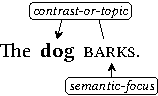
\includegraphics{pdf/the-dog-barks_g.pdf}} & & b. &
\evnup{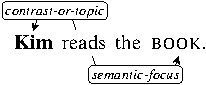
\includegraphics{pdf/kim-reads-the-book.pdf}} \\ c. &
\evnup{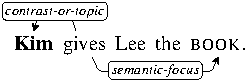
\includegraphics{pdf/kim-gives-lee-the-book.pdf}} & & d. &
\evnup{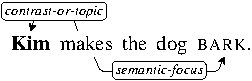
\includegraphics{pdf/kim-makes-the-dog-bark.pdf}} \\ e. &
\evnup{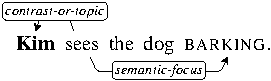
\includegraphics{pdf/kim-sees-the-dog-barking.pdf}} \\
\end{tabular}}}


Raising and control verbs have the same mapping type in
\tdl{info-str}; every dependent marked with respect to information
structure within a single clause has a co-index between its CLAUSE and
the INDEX of the semantic head in the clause (i.e.\ matrix clause
verb).\is{raising predicate}\is{control predicate}\is{CLAUSE}



\myexe{\eenumsentence{\toplabel{fig:verbal:rasing:control} 
\item \evnup{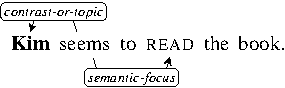
\includegraphics{pdf/kim-seems-to-read-the-book2.pdf}}
\item \evnup{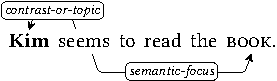
\includegraphics{pdf/kim-seems-to-read-the-book.pdf}}
\item \evnup{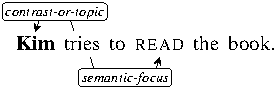
\includegraphics{pdf/kim-tries-to-read-the-book2.pdf}}
\item \evnup{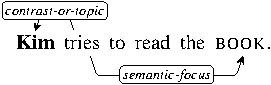
\includegraphics{pdf/kim-tries-to-read-the-book.pdf}}}}


\noindent For example, \textit{the \textsc{book}} in
(\ref{fig:verbal:rasing:control}b) is syntactically a complement of
\textit{read}, but is informatively bound to \textit{seems} whose
INDEX is connected to the INDEX in the clause.  Additionally, it is
interesting that \textit{Kim} has an \tdl{info-str} role in the matrix
finite clause,\is{\textit{info-str}} even though it is not the
semantic argument of \textit{seems}. The same goes for a control verb
\textit{try} in (\ref{fig:verbal:rasing:control}c--d).\footnote{As is
  well known, raising verbs (e.g.\ \textit{seem}, \textit{appear},
  \textit{happen}, \textit{believe}, \textit{expect}, etc.) and
  control verbs (e.g.\ \textit{try}, \textit{hope}, \textit{persuade},
  \textit{promise}, etc.) display several different properties, such
  as the semantic role of the subject, expletive subjects,
  subcategorization, selectional restriction, and meaning preservation
  \citep{kim:sells:08}. Nonetheless, they have
  \tdl{basic-icons-lex-item} in common as their supertypes, because
  they do not take tensed clauses as complements.}




Several verbal types take clausal complements as shown in
(\ref{fig:verbal:embedded}a) or clausal subjects as shown in
(\ref{fig:verbal:embedded}b), and these inherit from
\tdl{one-icons-lex-item}.

\myexe{\enumsentence{\toplabel{fig:verbal:embedded} 
\begin{tabular}[t]{ll}
a. & \evnup{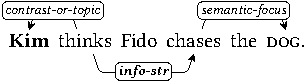
\includegraphics{pdf/kim-thinks-fido-chases-the-dog.pdf}} \\
b. & \evnup{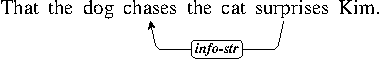
\includegraphics{pdf/that-the-dog-barks-surprises-kim.pdf}} \\
\end{tabular}}}




\noindent In (\ref{fig:verbal:embedded}a), the arrow from
\textit{chases} and \textit{dog} is locally established within the
embedded clause.  The \isi{binary relation} in the embedded clause
does not have to do with the main verb \textit{thinks}. The main verb
\textit{thinks} also has an arrow to the subject \textit{Kim} in the
local domain. The key point of this example is the arrow from the main
verb \textit{thinks} to the verb in the embedded clause
\textit{chases}. This arrow is introduced by element on the ICONS list
of \tdl{think} (\tdl{one-icons-lex-item}), and shows which information
structure relation the embedded clause has to the matrix
clause. Likewise, the arrow from \textit{surprises} and
\textit{chases} in (\ref{fig:verbal:embedded}b) represents the
inherent \tdl{info-str} element on the \isi{ICONS} list of
\textit{surprise}.


Both subjects and complements can be clausal at the same time.  In
these cases, it is necessary to inherit from \tdl{two-icons-lex-item}.
A typical example can be found in pseudo-clefts,\is{clefting}
including \textit{wh}-clefts, and inverted \textit{wh}-clefts as
exemplified in \myref{exe:verbal:triple}.\footnote{
  \myref{exe:verbal:triple} is originally taken from the ICE-GB
  (\citealt{nelson:etal:02}), and the expressions in angled brackets
  represent the indices of each sentence in the corpus.}  In
\myref{exe:verbal:triple}, the matrix verb \textit{is} inherently has
two elements of \tdl{info-str} on the \isi{ICONS}
list:\is{\textit{info-str}} The CLAUSE value of the first element is
its INDEX, and the TARGET is co-indexed with the INDEX of the verb in
the clausal subject (i.e.\ \textit{happened}). The CLAUSE of the
second is still linked to its INDEX, and the TARGET is co-indexed with
the INDEX of the verb in the complement
(i.e.\ \textit{caught}).\is{CLAUSE}




\myexe{\enumsentence{\label{exe:verbal:triple}
[What happened] is [they caught her without a
  license]. \ensuremath{<}S1A-078 \#30:2:A\ensuremath{>}}}




\noindent The dependency graph corresponding to
(\ref{exe:verbal:triple}) is presented in
\myref{fig:verbal:triple}. Note that the second arrow in
(\ref{exe:verbal:triple}) is specified as \tdl{focus}. That is, the
clausal complement in a \textit{wh}-cleft (e.g.\ \textit{they caught
  her without a license} in \ref{exe:verbal:triple}) is focused
\citep{kim:07}.\is{clefting} Since the other constituents cannot be
assigned \isi{focus}, the clausal subject in (\ref{exe:verbal:triple})
is specified as \tdl{non-focus}. The verbal entry \textit{is} includes
these values as lexical information.


\myexe{\enumsentence{\toplabel{fig:verbal:triple} 
\begin{tabular}[t]{ll}
\evnup{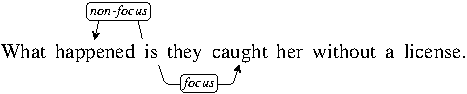
\includegraphics{pdf/wh-cleft1.pdf}}  \\
\end{tabular}}}





\subsubsection{Adjectives}
\label{10:sssec:adjectives}


Predicative adjective items are the same as the verbal items presented
thus far. The copula \textit{is} in \myref{exe:verbal:adj} is assumed
to be semantically and informatively empty, with the adjective
functioning as the semantic head of such sentences. This constraint is
specified in the following AVM, which passes up the CLAUSE-KEY of the
second argument (i.e.\ the adjective).\is{copula}

\myexe{\enumsentence{\label{avm:copula-verb-lex}
  \evnup{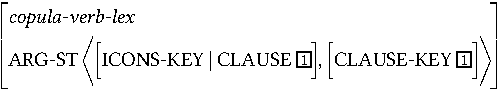
\includegraphics{pdf/copula-verb-lex.pdf}}}}


\noindent \textit{Happy} in (\ref{exe:verbal:adj}a) and \textit{fond
  of} in (\ref{exe:verbal:adj}b), which do not
constitute multiclausal constructions, inherit from
\tdl{basic-icons-lex-item}. Next, \textit{obvious} in
(\ref{exe:verbal:adj}c--d) takes clausal subjects, and \textit{sure}
and \textit{curious} in (\ref{exe:verbal:adj}e--f) take clausal
complements. These inherit from \tdl{one-icons-lex-item}.



\myexe{\eenumsentence{\label{exe:verbal:adj}
\item Kim is happy.
\item Kim is fond of apples.
\item That the dog barks is obvious.
\item It is obvious that the dog barks.
\item Kim is sure that the dog barks.
\item Kim is curious whether the dog barks.}}


\noindent There are also raising adjectives (e.g.\ \textit{likely})
and control adjectives (e.g.\ \textit{eager}), which, like raising and
control verbs, inherit from \tdl{basic-icons-lex-item}.\is{raising
  predicate}\is{control predicate}



Attributive adjectives are different in that they do not introduce the
\tdl{info-str} value that take their own event variable as the value
of CLAUSE.  Attributive adjectives and the nouns they are modifying
share the value of CLAUSE,\is{CLAUSE} which is co-indexed with the
INDEX of the verb heading the clause that they are part of.  For
example, the arrows on \textit{big} in \myref{fig:verbal:ajd} come
from the main verb of each sentence.  This linking strategy is
constructionally constrained by
\tdl{head-mod-phrase}. Section \ref{10:sec:monoclausal} gives an explanation
of how this linking is achieved via \tdl{head-mod-phrase}.






\myexe{\enumsentence{\toplabel{fig:verbal:ajd}
\begin{tabular}[t]{llllllll}
a. & \evnup{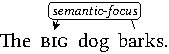
\includegraphics{pdf/the-big-dog-barks-1.pdf}} & &
b. & \evnup{
\includegraphics{pdf/kim-reads-the-big-book.pdf}} \\
\end{tabular}}}




There is a distinction between attributive and predicative adjectives
with respect to building up the list of ICONS, but there is no need to
use an extra lexical rule to discriminate them. What is of importance
is incrementally gathering \tdl{info-str} values into the list of
ICONS,\is{\textit{info-str}} and this strategy is achieved by phrase
structure rules, such as \tdl{head-comp-rule} for predicative
adjectives (as specified in the ARG-ST of \ref{avm:copula-verb-lex})
and \tdl{head-mod-rule} for attribute ones.



\subsubsection{Auxiliaries}
\label{10:ssssec:auxiliaries}





As far as \isi{ICONS} is concerned, auxiliaries in \ili{English} are divided
into two subtypes.\is{auxiliary} One contributes no predicate and no
\isi{ICONS} element, and thereby inherits from
\tdl{no-icons-lex-item}.  The other introduces an EP to RELS, and
thereby inherits from \tdl{basic-icons-lex-item}. Since complements of
auxiliaries are always non-finite, there are no auxiliaries of type
\tdl{one-icons-lex-item} or \tdl{two-icons-lex-item}.\is{auxiliary} An
example of the first category, \tdl{will} in (\ref{fig:verbal:aux}a)
is semantically empty, and does not occupy the INDEX of the
clause. Such an auxiliary, therefore, does not have any \tdl{info-str}
element in ICONS, either. Instead, the main verb, \textit{read} in
(\ref{fig:verbal:aux}a), has arrows to each of its dependents. By
contrast, \textit{can} in (\ref{fig:verbal:aux}b) introduces an EP to
RELS and has arrows to all individuals that introduce \tdl{info-str}
into the clause.\footnote{Its LKEYS{$\mid$}KEYREL{$\mid$}PRED is
  specified as ``\_can\_v\_modal\_rel'' in the ERG.}


\myexe{\enumsentence{\toplabel{fig:verbal:aux}
\begin{tabular}[t]{llllllll}
a. & \evnup{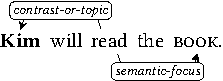
\includegraphics{pdf/kim-will-read-the-book.pdf}} & &
b. & \evnup{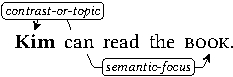
\includegraphics{pdf/kim-can-read-the-book.pdf}} \\
\end{tabular}}}

\noindent As stated above, these two types of auxiliaries inherit from
different lexical types.\is{auxiliary} \textit{Will} is an instance of
\tdl{no-icons-lex-item}, and therefore does not participate in the
articulation of information structure. Second, \textit{can} inherits
from \tdl{trans-first-arg-raising-lex-item-1} as represented 
in \myref{avm:trans-first-arg-raising-lex-item-1}. 
The CLAUSE value of
the subject (i.e.\ the first element in ARG-ST) is co-linked to its
own CLAUSE-KEY,\is{CLAUSE}\is{CLAUSE-KEY} and the second argument
(i.e.\ the VP) also shares the CLAUSE value with its own
CLAUSE-KEY.\footnote{Note that
  \myref{avm:trans-first-arg-raising-lex-item-1} actually contains
  more constraints, such as HCONS.}


\myexe{\enumsentence{\label{avm:trans-first-arg-raising-lex-item-1}
  \evnup{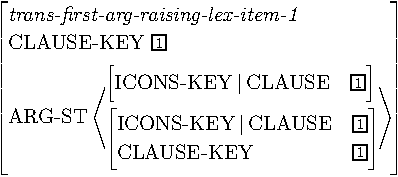
\includegraphics{pdf/trans-first-arg-raising-lex-item-1.pdf}}}}



The main verb which serves as the complement of modal auxiliaries can
sometimes take clausal complements.\is{auxiliary}\is{CLAUSE-KEY} In
this case, the CLAUSE-KEY is still occupied by the auxiliary as
sketched out in \myref{fig:can:embedded}:\is{\textit{info-str}} The
arrow to the verb in the embedded clause headed by \textit{chases} is
lexically introduced by \textit{think}, which inherits from
\tdl{one-icons-lex-item}. The CLAUSE-KEY of the second \tdl{info-str}
that \textit{think} introduces is still unbound in the VP
\textit{think Fido chases the dog}. Building up
\tdl{head-subj-phrase}, the CLAUSE-KEY that \tdl{chases} has in
relation to the matrix clause is finally co-indexed with the INDEX of
\textit{can}. Recall that the value of CLAUSE is bound when one clause
is identified (Section \ref{9:ssec:icons}). \tdl{Head-subj-phrase} serves to
identify which EP occupies the INDEX of the clause and fills in the
value of CLAUSE.





\myexe{\enumsentence{\label{fig:can:embedded}
\evnup{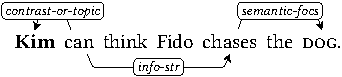
\includegraphics{pdf/kim-can-think-fido-chases-the-dog.pdf}}}}




\subsubsection{Copulae}
\label{10:sssec:cop}

Copulae, generally speaking, have at least three usages as exemplified
in \myref{exe:cop}.\is{copula} Note that some languages employ
lexically different copulae. For example, \ili{Korean} employs
\textit{i} as an ordinary copula and \textit{iss} as a locative
verb. To take another example, Mandarin \ili{Chinese} employs
\textit{sh\`{i}} as an ordinary copula and \textit{z\`{a}i} as a
locative verb. For this reason, I would use the three different names.

\myexe{\eenumsentence{\label{exe:cop}
\item Kim is the student. (identificational)
\item Kim is happy. (specificational)
\item Kim is in Seattle. (locative)}}


\noindent (\ref{exe:cop}a) can be paraphrased as \textit{Kim is
  identical to the student.}, while (\ref{exe:cop}b--c)
cannot. Traditionally, identificational copulae in many languages are
treated as ordinary transitive verbs, whose ARG-ST includes one NP for
the subject and the other NP for the complement (i.e.\ a two-place
predicate).  Thus, identificational copulae are assumed to be
contentful and thereby introduce an EP, whose
LKEYS{$\mid$}KEYREL{$\mid$}PRED value would be something like
``\_be\_v\_id\_rel''.


In contrast, the other two copula types are semantically empty items
that do not introduce any EP into the list of RELS in MRS.\is{MRS}
Thus, the semantic heads of (\ref{exe:cop}b--c) are respectively
computed as \textit{happy} and \textit{in}. 
Since the locative verb is not semantically void in such a
language, the lexical entry for the locative verb has a PRED value
like ``\_be+located\_v\_rel''.



Identificational copulae inherit from \tdl{basic-icons-lex-item},
while the others inherit from \tdl{no-icons-lex-item}. That means
semantic heads that occupy the INDEX of the clauses in
(\ref{exe:cop}b--c) are \textit{happy} and \textit{in},
respectively.\is{CLAUSE-KEY} In other words, the CLAUSE-KEY in
(\ref{exe:cop}b--c) is linked to the INDEX of \textit{happy} and
\textit{in}. (\ref{fig:verbal:cop}a--c) represent the information
structure of (\ref{exe:cop}a--c), respectively.

\myexe{\enumsentence{\toplabel{fig:verbal:cop} 
\begin{tabular}[t]{ll}
a. & \evnup{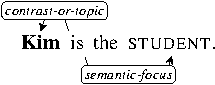
\includegraphics{pdf/kim-is-the-student.pdf}}\\
b. & \evnup{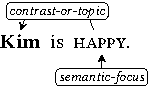
\includegraphics{pdf/kim-is-happy.pdf}} \\
c. & \evnup{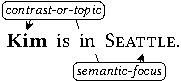
\includegraphics{pdf/kim-is-in-seattle.pdf}} \\
\end{tabular}}}



\subsection{Adpositions}
\label{10:ssec:adpositions}


Adpositions normally inherit from either \tdl{basic-icons-lex-items}
or \tdl{one-icons-lex-item}.\is{adposition} Every
information-structure marking adposition inherits from
\tdl{one-icons-lex-item}.  If an adposition does not contribute to
information structure, it inherits from \tdl{basic-icons-lex-item}.
Adpositions that inherit from \tdl{basic-icons-lex-items} can have an
\isi{ICONS} element introduced later when another means of marking
information structure (e.g.\ an accent on \textit{under} in
\ref{exe:prep}b) is used.



\myexe{\enumsentence{\label{exe:prep}
\begin{tabular}[t]{ll}
Q: & {Did Kim put the book \underline{on} the desk?}\\
A: & {No. Kim put the book \underline{under} the desk.}\\
\end{tabular}}}


Prepositions in \ili{English} do not inherit from
\tdl{one-icons-lex-items}, because there is no information-structure
marking preposition in English.  \ili{Japanese} has both types. As
discussed thus far, information-structure marking postpositions, such
as {\ga} (nominative) and \textit{o} (accusative) and {\wa} (contrast
or topic),\is{contrast}\is{topic} are instances of
\tdl{one-icons-lex-item}. That means they introduce one element into
the \isi{ICONS} list. The TARGET of the \isi{ICONS} element is
co-indexed with the INDEX of their complement (i.e.\ XP that they are
attached to), and the ICONS-KEY of each postposition is lexically
specified:\is{ICONS-KEY} \tdl{non-topic} for {\ga} and \textit{o},
\tdl{contras-or-topic} for \wa.  Other than these, \isi{focus}
particles syntactically classified as postpositions in Japanese are
also instances of \tdl{one-icons-lex-item}.  These include
\textit{dake} `only', \textit{shika} `except', \textit{mo} `also', and
so on \citep{hasegawa:11,hasegawa:koenig:11}. They behave in the same
manner as {\ga}, \textit{o}, and {\wa}, but their \tdl{info-str} value
is \tdl{focus}.\is{\textit{info-str}} Other postpositions that do not
mark information structure in Japanese inherit from
\tdl{basic-icons-lex-item}. These include \textit{made} `till',
\textit{kara} `from', etc.





\subsection{Determiners}
\label{10:sssec:determiners}


Determiners inherit from either \tdl{one-icons-lex-item} or
\tdl{basic-icons-lex-item}, depending on whether or not they mark
information structure by themselves.  \ili{English} does not have
determiners that inherit from \tdl{one-icons-lex-item}, because there
is no information-structure marking determiner.  It is reported that
some languages employ information-structure marking determiners. For
example, \ili{Lakota} (a Siouan language spoken in Dakota) uses a
definite determiner \textit{\textipa{k'u\ng}}
to signal \isi{contrastive topic}.\footnote{Section \ref{13:ssec:lc-lang}
provides more explanation about
  \textit{\textipa{k'u\ng}} in Lakota \mypage{13:ssec:lc-lang}.}
These determiners inherently include an \isi{ICONS} element
(i.e.\ \tdl{one-icons-lex-item}).


Determiners in \ili{English} may bear the A-accent as shown in
\myref{exe:det}.\is{A-accent}

\myexe{\eenumsentence{\label{exe:det}
\item Kim reads \textsc{the} book.
\item Kim reads \textsc{some}/\textsc{all} books.}}

\noindent Notice that \tdl{focus} is assigned to the nouns, not the
determiners themselves. That is, the focused items in \myref{exe:det}
are \textit{book}(\textit{s}), not the determiners.  Thus, when a
determiner has an \isi{ICONS} element, its TARGET should be co-indexed
with the INDEX of the NP.\is{A-accent} \is{B-accent} For example, the
A-accented \textsc{all} in (\ref{exe:det}b) is constrained as
follows.\footnote{The current analysis employs two hypothetical
  suffixes (\textit{-a} for the A-accent and \textit{-b} for the B-accent) and the
  suffixes are attached by lexical rules. Two lexical rules presented
  in \myref{avm:fc:tp:eng} later take nominal and verbal items as
  their daughter.\is{B-accent} In addition to them, there could be one
  more lexical rule that takes determiners as their daughter. These
  rules are not presented in the current analysis.}


\myexe{\enumsentence{\label{avm:all}\evnup{
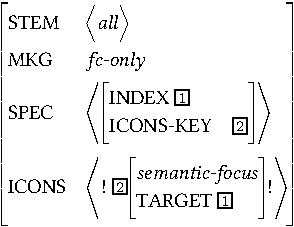
\includegraphics{pdf/all.pdf}}}}

\noindent Notably, the \tdl{info-str} value that determiners assign to
the specified NPs should be consistent with the ICONS-KEY of the
NPs;\is{ICONS-KEY} for example, `\textsc{the} \textbf{book}' is
ill-formed,\is{semantic focus} because the \tdl{semantic-focus} that the determiner
involves is inconsistent with the \tdl{contrast-or-topic} the noun
carries.\footnote{Section \ref{10:sssec:quantifiers} provides more discussion
  on information structure values of
  quantifiers \mypage{10:sssec:quantifiers}.\is{quantifier}}




\subsection{Adverbs}
\label{10:ssec:adverbs}


Adverbs cross-linguistically inherit from \tdl{basic-icons-lex-item}.
\myref{fig:adv} is illustrative of the information structure relation
that adverbs have within a clause. Just as with attributive
adjectives, the relation is bound to the HOOK{$\mid$}INDEX of the
semantic head within the clause.


\myexe{\enumsentence{\toplabel{fig:adv}
\begin{tabular}[t]{llllllll}
a. & \evnup{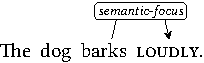
\includegraphics{pdf/the-dog-barks-loudly.pdf}} & &
b. & \evnup{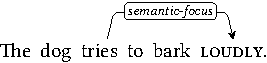
\includegraphics{pdf/the-dog-tries-to-bark-loudly.pdf}} \\
\end{tabular}}}




\subsection{Conjunctions}
\label{10:sssec:conjunctions}














First of all, all conjunctions that take adverbial clauses as their
complement inherit from
\tdl{one-icons-lex-item}.\is{TARGET}\is{CLAUSE-KEY}\is{adverbial
  clause} They have their CLAUSE-KEY linked to the INDEX of the main
clause's semantic head. Note that the semantic head of the matrix
clause is co-indexed with the element in HEAD{$\mid$}MOD.  They also
have their TARGET linked to the INDEX of their complement (i.e.\ the
semantic head of the adverbial clause).


\myexe{\enumsentence{\label{avm:subconj-word:ch10-1}
\evnup{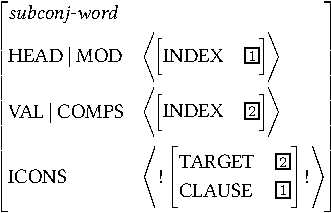
\includegraphics{pdf/subconj-word.pdf}}}}

\noindent Second, conjunctions that involve temporal adverbial
clauses, such as \textit{when}, \textit{before}, and \textit{after},
are related to \tdl{topic}, if they appear before the main clause
\citep{haiman:78}.  That means that the information structure value
between the two semantic heads should be \tdl{topic}. This value is
assigned by the temporal conjunctions themselves.  Third, conditional
conjunctions (e.g.\ \textit{if} and \textit{unless} in \ili{English})
also assign \tdl{topic} to the element in ICONS
\citep{ramsay:87}.\footnote{Section \ref{10:ssec:adjunct} provides more
  information about temporal and conditional
  conjunctions \mypage{10:ssec:adjunct}.}\is{topic}  Fourth, causal
conjunctions, such as \textit{because} in English, and \textit{weil}
in German, differ by language with respect to information structure
relation to the matrix clause \citep{heycock:07}. Therefore, their
information structure value is language-specifically
constrained.\is{\textit{info-str}} That is, causal conjunctions in
some languages (e.g.\ English) have an \isi{ICONS} element whose value
is \tdl{info-str}, while similar conjunctions in other language might
have an \isi{ICONS} element whose value is more specific.










Coordinating conjunctions, such as \textit{and} and \textit{or}, are
another story. First, each coordinand can have its own information
structure relation to the semantic head in the clause if it is marked
with respect to information structure.  Second, coordinands in a
single coordination may have different information structure values
from each other. For example, \textit{Kim} and \textit{\textbf{Sandy}}
in (\ref{exe:coord:contrast}B) have the same status in the syntax of
coordination, but \textit{\textbf{Sandy}} is contrastively focused as
vetted by the correction test. In this case, while \textit{Kim}
introduces no \isi{ICONS} element, \textit{\textbf{Sandy}} introduces
an \isi{ICONS} element and the element is assigned
\tdl{contrast-or-topic} by the B-accent.\is{contrastive focus}



\myexe{\enumsentence{\label{exe:coord:contrast}
\begin{tabular}[t]{ll}
A: & {Kim and Lee came.}\\
B: & {No. Kim and \textbf{Sandy} came.}\\
\end{tabular}}}


\noindent Third, the coordinate phrase itself also can have an
information structure relation to the semantic head. For instance, the
fronted constituent in \myref{exe:coord:eng} (specified as
\tdl{focus-or-topic}) is a coordinate phrase.  



\myexe{\enumsentence{\label{exe:coord:eng}
    The book and the magazine, Kim read.}}


\noindent In this case, an ICONS
element that indicates the information structure relation between the
coordinate phrase \textit{The book and the magazine} and the main verb
\textit{read} is added into C-CONT{$\mid$}ICONS.\footnote{Information
  structure in coordinated phrases would be an interesting research
  \isi{topic}. In particular, since the 
  \lingo \isi{Grammar Matrix} system includes a
  library of coordination, this idea needs to be implemented and
  tested though it is left to future work.}



\section{Phrasal types}
\label{10:sec:monoclausal}


Information structure can also be restricted by phrase structure
rules.  Phrasal types can be roughly divided into \tdl{unary-phrase}
and \tdl{binary-phrase}. First, \isi{ICONS} is an accumulator list:
\isi{ICONS} is implemented as a \tdl{diff-list}, and the elements are
gathered up the tree using \tdl{diff-list} append. Second, the
information-structure related features (e.g.\ MKG and
L/R-PERIPH)\is{MKG} are shared between mother and daughter in a
\tdl{unary-phrase}, with no further
constraint.\is{L-PERIPH}\is{R-PERIPH} For instance, \tdl{unary-phrase}
is defined as in \myref{avm:unary}. \isi{L-PERIPH} and \isi{R-PERIPH}
in \myref{avm:unary} have not yet been mentioned. They impose an
ordering constraint on constituents with respect to expressing
information structure. Section \ref{9:ssec:periphery} discusses how
they contribute to constraining information structure at the phrasal
level.


\myexe{\enumsentence{\label{avm:unary}
  \evnup{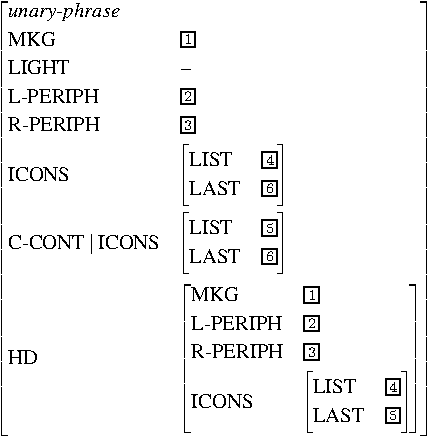
\includegraphics{pdf/unary-phrase.pdf}}}}



Third, there are five basic subtypes of \tdl{binary-headed-phrase}:
(i) \tdl{basic-head-subj-phrase}, (ii) \tdl{basic-head-comp-phrase},
(iii) \tdl{basic-head-spec-phrase}, (iv)
\tdl{basic-head-mod-phrase-simple}, and (v)
\tdl{basic-head-filler-phrase}. The first three (i-iii) are the same
as the previous versions, but with [C-CONT{$\mid$}ICONS
  \ensuremath{<}!  !\ensuremath{>}] added.  The empty \tdl{diff-list}
in \mbox{C-CONT{$\mid$}ICONS} means that these rules never contribute
\isi{ICONS} elements.  \tdl{Basic-head-mod-phrase-simple} is further
constrained as follows:\is{ICONS-KEY} The ICONS-KEY{$\mid$}CLAUSE and
CLAUSE-KEY of NON-HEAD-DTR has a coreference with the
ICONS-KEY{$\mid$}CLAUSE of HEAD-DTR.\is{CLAUSE}\is{ICONS-KEY} That
means the modifier and the modificand share the same CLAUSE-KEY. The
ICONS-KEY and CLAUSE-KEY indicate in which clause the adjunct is
focused or topicalized.  Additionally, an empty \isi{ICONS} list is
added.


\myexe{\enumsentence{\label{avm:head-mod-phrase}
  \evnup{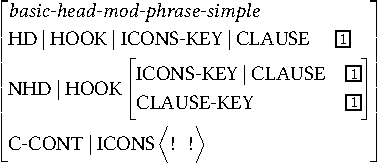
\includegraphics{pdf/head-mod-phrase.pdf}}}}


\noindent Finally, \tdl{basic-head-filler-phrase} does not include
\mbox{[C-CONT{$\mid$}ICONS \ensuremath{<}!  !\ensuremath{>}]}, because
this phrase may or may not contribute ICONS
elements. Section \ref{11:ssec:phr} provides an explanation of its role in
configuring information structure. Related constructions include
clause-initial/final \isi{focus} constructions, focus/\isi{topic}
\isi{fronting}, and so forth.



\section{Additional constraints on configuring information structure}
\label{9:sec:other-constraints}

Other than the hierarchical constraints presented in the previous
chapter, there must be some additional constraints in order to
implement information-structure related phenomena within the \lingo
\isi{Grammar Matrix} system.  L/R-PERIPH in Section \ref{9:ssec:periphery}
and LIGHT in Section \ref{9:ssec:lightness},\is{lightness} as flag features,
impose a constraint on the position of components of information
structure. The former is newly introduced, while the latter had
already been implemented in the system. PHON in
Section \ref{9:ssec:phonology}, newly introduced, is adapted from
\citet{bildhauer:07}.


\subsection{Periphery}
\label{9:ssec:periphery}


As surveyed in Chapter~\ref{chapter4}, syntactic positioning is one
method of expressing information structure.\is{periphery}\is{syntactic
  positioning} The positions associated with \isi{focus} include (i)
\isi{clause-initial} (e.g.\ in \ili{Akan}, \ili{Ingush},
\ili{Yiddish}, etc.), (ii) \isi{clause-final} (e.g.\ in \ili{Russian},
\ili{Bosnian Croatian Serbian}, etc.), (iii) \isi{preverbal} (e.g.\ in
\ili{Hungarian}, \ili{Basque}, \ili{Turkish}, etc.), and (iv)
\isi{postverbal} (e.g.\ in \ili{Portuguese}, \ili{Chiche{\^w}a},
etc.). The common position for topics is sentence-initial though some
languages (e.g.\ \ili{Danish}) do not use the initial positions to
signal \isi{topic}.


In order to implement constraints on periphery, the present study
suggests the use of two flag features that constrain the first two
\isi{focus} positions (i.e.\ (i) L-PERIPH for clause(sentence)-initial
focus and (ii) R-PERIPH for clause-final
focus).\is{clause-initial}\is{clause-final}\is{L-PERIPH}\is{R-PERIPH}
The remaining two positions, including (iii) \isi{preverbal} and (iv)
\isi{postverbal}, are constrained by the feature called
LIGHT,\is{lightness} discussed in Section \ref{9:ssec:lightness}.
Even though flag features are related to syntax and semantics, they
take part in syntactic configuration and semantic computing only in an
indirect way. They are traditionally located directly under
SYNSEM. This tradition holds L/R-PERIPH. Additionally, although their
value type is \tdl{luk}, they are usually constrained as + or --
(i.e.\ \tdl{bool}).



\mbox{[L-PERIPH +]} indicates that a constituent with this feature
value cannot be combined with another constituent leftward. [R-PERIPH
  +] likewise indicates there must be no other constituent to the
right of a constituent marked as such.  In other words, a constituent
marked as [L/R-PERIPH +] has to be peripheral in word order unless
there is an exceptional rule.  A constituent with [L-PERIPH +]
should be in the left-most position within a given clause
(i.e.\ clause-initial).\is{clause-initial}  A constituent that is
[R-PERIPH +] should be in the right-most position, in other
words clause-final.\is{L-PERIPH}\is{R-PERIPH}\is{clause-final}


One of the representative cases in which both features are required
can be found in Russian, which places contrastively focused
constituents in the clause-initial position and non-contrastively
focused ones in the clause-final position
\citep{neeleman:titov:09}.\is{clause-initial}\is{clause-final}\is{non-contrastive focus}
Thus, the clause-initial constituent (\tdl{contrast-focus}) is
\mbox{[L-PERIPH +]}, and the clause-final constituent
(\tdl{semantic-focus}) is \mbox{[R-PERIPH +]}.\is{contrastive focus}\is{semantic focus}
\ili{Russian} has several more examples that clearly interact with periphery: Russian employs a
clitic \textit{li}, which should appear in the second position of an
utterance \citep{gracheva:13}.\footnote{According to
  \citet{gracheva:13}, there is one more constraint on \textit{li}:
  The sentence should be interrogative. That is, the sentential force
  of the utterance is conditioned as \mbox{[SF \tdl{ques}]} by
  \tdl{li}.} This clitic modifies the immediately preceding
constituent (i.e.\ the most left-peripheral item), and sometimes
assigns \tdl{contrast-focus} to it, depending on the part of speech of
the constituent it attaches to and context.\is{periphery} Notably,
\textit{li} imposes the \mbox{[L-PERIPH +]} constraint on left-located
constituents. For example, the emphasized constituents in
\myref{exe:rus:varya:li} can be evaluated as containing
\tdl{contrast-focus}.


\myexe{\eenumsentence{\toplabel{exe:rus:varya:li}
\item \shortex{5}
{\myemp{Na rynke} & li & Ivan & kupil & popugaya?}
{On market-\textsc{prep} & li & Ivan-\textsc{nom} & buy-\textsc{pst.sg.m} & parrot-\textsc{acc}}
{`Was it \myemp{in the market} that Ivan bought a parrot?'}
\item \shortex{5}
{\myemp{Govoriashego} & li & popugaja  & kupil &Ivan?}
{Talking-\textsc{sg.masc.acc} & li & parrot-\textsc{acc} & buy-\textsc{pst.sg.m} & Ivan-\textsc{nom}}
{`Did Ivan buy a \myemp{talking} parrot?' [rus]}}}


\noindent \citet{gracheva:13} provides other clitics that potentially
signal information structure meanings in Russian, of these
\textit{-to}, \textit{\v{z}e}, and \textit{ved'} also interact with
the periphery of their modificands in a similar way.\footnote{Russian
  has been known to employ pragmatically conditioned word order
  \citep{rodionova:01}. In that case, the pragmatic condition largely
  refers to information structure. For the reason, it seems that a
  variety of means are used for expressing information structure in
  Russian.}  These findings indicate that L-PERIPH and R-PERIPH play
an important role in configuring information structure in Russian-like
languages.\is{L-PERIPH}\is{R-PERIPH}


\isi{L-PERIPH} can also be used for imposing a restriction on the
position of topics in topic-first languages (e.g.\ \ili{Japanese} and
\ili{Korean}).  The left-most (i.e.\ sentence-initial) and probably
\isi{topic}-marked constituent in topic-first languages should be
\mbox{[L-PERIPH +]} disallowing the appearance of any constituents to
its left.  One exceptional case to this restriction is
\tdl{frame-setting}, because a series of constituents functioning as
frame-setters can show up in the sentence-initial position. This is a
phenomenon which seems language-universal
\citep{li:thompson:76,chafe:76,lambrecht:96}. Now that
\tdl{topic-comment} and its subtypes have an additional constraint on
L-PERIPH, the AVMs offered in
Section \ref{9:ssec:sform} \mypage{avm:frame-setting} are extended as
follows.\is{frame-setting} The more specific rules that inherit from
these will be presented in
Section \ref{10:sec:scrambling} \mypage{avm:topic-comment:3} with specific
examples of articulating the \isi{scrambling} constructions in
Japanese and Korean.

\myexe{\eenumsentence{\toplabel{avm:topic-comment:2}
\item\evnup{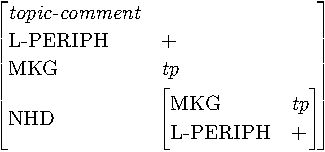
\includegraphics{pdf/topic-comment2.pdf}}
\item\evnup{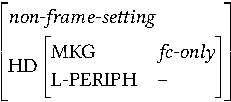
\includegraphics{pdf/non-frame-setting2.pdf}}}}




L-PERIPH also plays a role in \isi{focus}/topic \isi{fronting}
constructions.\is{L-PERIPH} If a language places focused constituents
in the clause-initial position and also has the \isi{topic}-first
restriction,\is{clause-initial} the fronted constituents are
associated with \tdl{focus-or-topic}, as suggested
before. \ili{Yiddish} typically exhibits such a behavior as in
\myref{exe:ydd}.  Yiddish is a V2 language with a neutral word order
of SVO, in which the verb (i.e.\ the syntactic head in a sentence)
should occur in the second position of the linear order
\citep{jacobs:05}. Therefore, if the object is focused in Yiddish, the
linear order, as exemplified (\ref{exe:ydd}b), should be OVS, not
OSV.\is{clefting} The same goes for sentences in which adverbials are
fronted as shown in (\ref{exe:ydd}c--d).\footnote{In fact, the
  translations in \myref{exe:ydd} provided by \citet{jacobs:05} follow
  the notion that the focused XPs in cleft constructions exhibit
  exhaustive inferences (i.e.\ contrastive
  meaning).\is{contrast} Chapter~\ref{chapter10-3} addresses this interpretation in
  detail (Section \ref{10:sec:clefts}).}


\myexe{\eenumsentence{\label{exe:ydd}
\item\shortexnt{5} 
{Der ler{\textschwa}r & \v{s}rajbt & di zacn & mit krajd & afn tovl.}
{The teacher & writes & the sentences & with chalk & on the blackboard (neutral)}
\item\shortex{5} 
{Di zacn  & \v{s}rajbt & der ler{\textschwa}r & mit krajd & afn tovl.}
{the sentences & writes & the teacher & with chalk & on the blackboard}
{`It's the sentence (not mathematical equations) that the teacher is writing with chalk on the blackboard.'}
\item\shortex{5} 
{mit krajd &  \v{s}rajbt & der ler{\textschwa}r & di zacn & afn tovl.}
{with chalk & writes & the teacher & the sentences & on the blackboard}
{`It's with chalk (not with a crayon) that that the teacher is writing the sentence on the blackboard.'}
\item\shortex{5} 
{afn tovl & \v{s}rajbt & der ler{\textschwa}r & di zacn &  mit krajd.}
{on the blackboard & writes & the teacher & the sentences & with chalk}
{`It's on the blackboard (not the notepad) that that the teacher is writing the sentence with chalk.' [ydd] \citep[224]{jacobs:05}}}}



\noindent Note that (\ref{exe:ydd}a) is ambiguous (See Section
\ref{4:sec:syntactic}). This is like ordinary \isi{focus}/\isi{topic}
\isi{fronting} constructions in other languages. However, in either
case the focused or topicalized constituent should be first, and is
constrained as \mbox{[L-PERIPH +]}.



\subsection{Lightness}
\label{9:ssec:lightness}


Preverbal and \isi{postverbal} \isi{focus} positions are constrained by
LIGHT,\is{lightness} which already existed in the \lingo \isi{Grammar
  Matrix} core (i.e.\ \texttt{matrix.tdl}) in order to distinguish
words from phrases.\is{preverbal} Using LIGHT for discriminating words
and phrases is inspired by the ``Lite'' feature
\citet{abeille:godard:01}
suggest.\footnote{\citet[54]{crowgey:bender:11} also make use of
  this feature to impose a constraint on negation in
  Basque:\is{lightness} ``The feature LIGHT is defined on synsems with
  a value \textit{luk}. Lexical items are [LIGHT +], while phrases are
  \mbox{[LIGHT --]}. This stipulation ensures that the verbal complex
  rule applies before the auxiliary picks up any arguments in any
  successful parse.''\is{auxiliary}} LIGHT is located directly under
SYNSEM because it is a flag feature.


[LIGHT +] is attached to words, while [LIGHT --] is attached to
phrases. The value of LIGHT, whose type is \tdl{luk}, is sometimes
co-indexed with that of HC-LIGHT originally taken from the ERG. HC
stands for Head-Complement. The purpose of using HC-LIGHT is to
indicate whether a \tdl{head-comp-phrase} projected from a head is
regarded as light or heavy. If an element in a parse tree has
\mbox{[LIGHT +]},\is{lightness} it indicates the element has not yet
been converted into an instance of a phrasal type. As for verbal nodes
in parse trees, the distinction between V and VP is naturally made by
the value of LIGHT.



Preverbal and \isi{postverbal} foci are always realized as
\tdl{narrow-focus} presented in the previous
chapter \mypage{avm:narrow-focus}.\is{preverbal}\is{narrow focus} In addition to this
constraint, I argue that \isi{preverbal} and \isi{postverbal} focus
can be combined only with Vs that are \mbox{[LIGHT +]}.  \ili{Basque},
for instance, is known for the preverbal focus position.  In the
Basque sentence below, \textit{Jonek} `Jon' is signaled as
\tdl{focus}, which is immediately followed by \textit{irakurri du}
`read has'.





\myexe{\enumsentence{\label{exe:urbina:focus:ch10-1}
\shortex{4}
{Eskutitza, & Jonek & irakurri & du}
{letter & Jon & read & has}
{`\textsc{Jon} has read the letter.' [eus] \citep[312]{urbina:99}}}}



My analysis of the sentence is as follows: The auxiliary verbal item
\textit{du} `has' takes \textit{irakurri} `read' as its complement,
but combination is still regarded as a word rather than a phrase. That
is, \textit{irakurri du} is \mbox{[HC-LIGHT +]},\is{lightness} and
shares a coreference with LIGHT.  \textit{Jonek} then combines with
\textit{irakurri du} (which is still [LIGHT +]), constituting a
\tdl{head-subj-phrase}. Because the \tdl{head-subj-phrase}
(i.e.\ \textit{Jonek irakurri du}) is now \mbox{[LIGHT --]}, no more
\isi{preverbal} foci can take place.  \citet{crowgey:bender:11}
provide a similar analysis. They argue that Basque has a constraint
like \myref{def:joshua} with respect to the variation of word order.

\myexe{\enumsentence{\label{def:joshua} If the lexical verb is to the
    left of the auxiliary, then the lexical verb must be left-adjacent
    to the auxiliary. \citep[49]{crowgey:bender:11}}}


\noindent This constraint explains the ungrammaticality of
\myref{exe:joshua:10-3}, in which the main verb and the auxiliary are
not adjacent to each other.\is{auxiliary} This is further evidence
that a main verb plus an auxiliary (e.g.\ \textit{irakurri du}) behave
as a single [LIGHT +] (in other words non-phrasal) verbal constituent.

\myexe{\enumsentence{\label{exe:joshua:10-3}
\shortex{4}
{*Liburu & irakurri & Mirenek & du}
{book.\textsc{abs.sg} & read.\textsc{perf} & Mary.\textsc{erg.sg} & \textsc{3sgO.pres.3sgA}}
{`Mary has read a book.' [eus] \citep[48]{crowgey:bender:11}}}}



For more explanation about constraints on \isi{preverbal} and
\isi{postverbal} foci, two pseudo sentences in Language \textit{A}
(presented in Section \ref{9:ssec:sform}) can be instantiated as shown
in \myref{exe:lang-a:2}. If Language \textit{A}, whose word-order
properties are repeated in \myref{def:lang-a:ch10-1}, has ditransitive
verbs, and the ordinary order between objects is [indirect object
  (\textit{iobj}) + direct object (\textit{dobj})], then
(\ref{exe:lang-a:2}a) is in the basic word order.

\myexe{\eenumsentence{\label{def:lang-a:ch10-1}
\item Language \textit{A} employs SVO as its basic word order.
\item Focused constituents in Language \textit{A} are realized in the immediate
  preverbal position.
\item Additionally, there is an optionally used accent, which
  expresses focus.}}

  
\myexe{\eenumsentence{\label{exe:lang-a:2}
\item subj verb iobj dobj. (neutral)
\item subj dobj verb iobj. (focus on dobj)}}



\noindent A sample derivation for (\ref{exe:lang-a:2}b) in which the
direct object is focused and \isi{preverbal} is illustrated below.


\myexe{\enumsentence{\label{fig:lang-a:2}\evnup{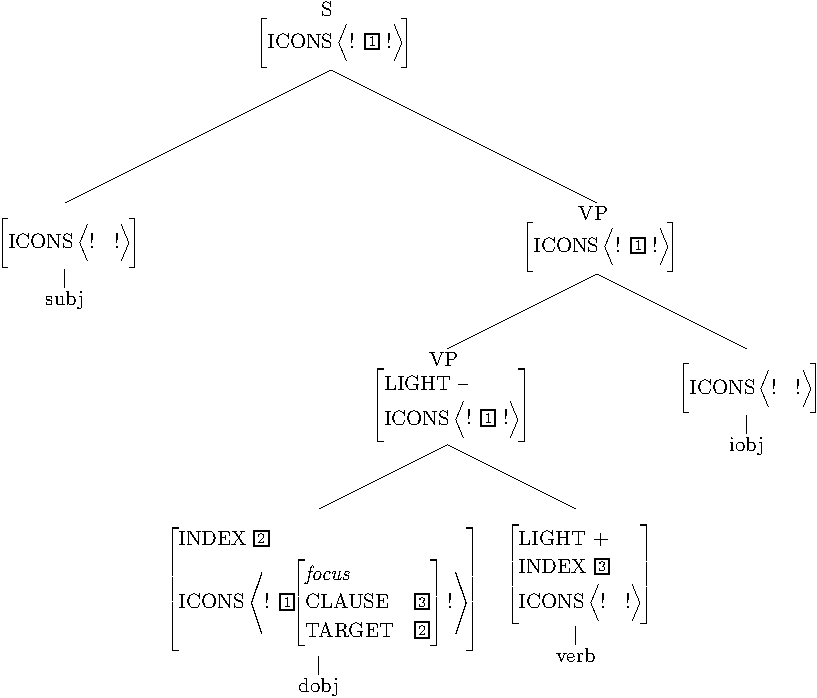
\includegraphics[width=.9\textwidth]{pdf/lang-a2.pdf}}}}


\noindent The focused item \textit{dobj}, which is not in
  situ, is combined with a [LIGHT +] verb before anything else. They
constitutes a \tdl{head-comp-phrase}, which is now [LIGHT --]. Next,
the VP takes \textit{iobj}, which is in situ, as the second
complement, and forms another VP as \tdl{head-comp-phrase}. Finally,
the subject is combined with the second VP into a
\tdl{head-subj-phrase}.  In this case, the first and the second
\tdl{head-comp-phrase} are realized as two different rules. The first
one puts constraints on both the NON-HEAD-DTR (e.g.\ \textit{dobj} in
\ref{exe:lang-a:2}b) and the HEAD-DTR (e.g.\ \textit{verb}); an
information structure value \tdl{focus} is assigned to the
NON-HEAD-DTR and the HEAD-DTR required to be [LIGHT +].\is{lightness}
The second one does not signal any specific values of information
structure, but requires the HEAD-DTR to be [LIGHT --]. Notably, this
analysis is not applied to sentences in the neutral word order. For
example, \textit{subj} in (\ref{exe:lang-a:2}a) is in the immediately
preverbal position, but it is in situ in the neutral word
order. Thus, it is not necessarily analyzed as containing
\tdl{focus}.\is{focus}





\subsection{Phonological structure}
\label{9:ssec:phonology}


The phonological structure proposed by \citet{bildhauer:07} is not
completely applied to the customization system as is, because the
phonological behaviors in many languages remain hitherto unknown.  As
far as the \lingo \isi{Grammar Matrix} system is concerned, the
phonological structure itself is implemented into \texttt{matrix.tdl}
in \isi{TDL}, but no further rules are implemented.  Crucially a set
of phonology-related features are now implemented in
\texttt{matrix.tdl} and available for use by future developers of
Matrix-derived grammars.


\citet{bildhauer:07} proposes four levels of phonological structure,
consisting of (i) prosodic word, (ii) phonological phrase, (iii)
intonational phrase, and (iv) phonological utterance, and two
intonational typed feature structures, including (v) pitch accents,
and (vi) boundary tones. Among them, the present study is not
concerned with the first three structures, because it is difficult to
obtain an acoustic system to resolve the prosodic levels reliably.  In
other words, the rules presented in Chapter~\ref{chapter8}
\mypage{avm:bildhauer:rules} are tentatively disregarded in the
current work. The last three are largely related to \isi{focus
  projection}, but the rules for them are also altered to be suitable
for implementation. The altered rules, such as the focus-prominence
rule and focus-projection rule, are presented in
Chapter~\ref{chapter10-4} which is especially concerned with how to
calculate the spreading of \isi{focus}.


Prosodic patterns in \ili{Japanese} and \ili{Korean}, with respect to
information structure, have been substantially revealed by phonetic
experiments \citep{jun:etal:07,ueyama:jun:98,jun:lee:98}. Prosodic
behaviors of information structure in \ili{Spanish} are
well-summarized in \citet{bildhauer:07} as well. Yet, the present
study has little interest in them, because the main purpose of the
current work is to create a grammar library for information structure
in the \lingo \isi{Grammar Matrix} system. The system is built for
text-based processing, and has not yet reflected phonological
information in a significant manner. It is left to the future research
to implement prosodic rules in \ili{Japanese}, \ili{Korean},
\ili{Spanish}, and other languages.






\section{Sample derivations}
\label{9:sec:samples}



This section provides sample derivations, which briefly show how
information structure works with \isi{ICONS} in several different types of
languages. The languages that this section presents are \ili{English},
\ili{Japanese}, \ili{Korean}, and \ili{Russian}.\is{ICONS-KEY} The type of the
ICONS-KEY value of a constituent, which points to an element of the
\isi{ICONS} list, can be constrained by (i) accents responsible for
information structure meanings, (ii) lexical rules attaching
information structure marking morphemes, (iii) particles like
\ili{Japanese} \textit{wa} combining as heads or modifiers with NPs,
and/or (iv) phrase structure rules corresponding to distinguished
positions.





\subsection{English}
\label{9:ssec:eng}

Pitch accents primarily serve to express information structure
meanings in \ili{English} as shown in \myref{exe:sample:derivation:eng}.

\myexe{\enumsentence{\toplabel{exe:sample:derivation:eng}
\begin{tabular}[t]{ll}
a. & {The \textsc{dog} barks.}\\ 
b. & {The \textbf{dog} barks.}\\
\end{tabular}}}

In other words, English imposes a constraint on the A and B
accents. In the current work, they are hypothetically realized as
suffixes (e.g. \textit{-a}, \textit{-b}), whose lexical rules are provided in
(\ref{avm:fc:tp:eng}a--b). That is,
(\ref{exe:sample:derivation:eng}a--b) are actually encoded into
\textit{The dog-a barks.} and \textit{The dog-b barks.}  respectively
as an input string for parsing and an output string from generation.




UT{$\mid$}DTE, adapted from \citet{bildhauer:07}, aims to calculate
\isi{focus projection} in Chapter~\ref{chapter10-4}
(Section \ref{10:sec:f-marking}). The current work gives the value of
UT{$\mid$}DTE a coreference with that of MKG{$\mid$}FC, because focus
projection is not always licensed by prosodic means across languages
\citep{choe:02}.\is{MKG} This means that MKG{$\mid$}FC is responsible
for spreading the \isi{focus} domain to larger phrases, and the value should
be the same value as the value of UT{$\mid$}DTE in \ili{English}.

\myexe{\enumsentence{\toplabel{avm:dte} 
\evnup{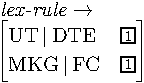
\includegraphics{pdf/lex-rule.pdf}}}}




Next, (\ref{avm:fc:tp:eng}a--b) are the lexical rules for A and B
accents. Each of their PA values, taken from
\citeauthor{bildhauer:07}'s hierarchy
\myref{fig:bildhauer:tone-or-none}, stands for H* and L+H* in the ToBI
format, respectively.\is{A-accent}\is{B-accent} MKG for the A-accent
is valued as \tdl{fc-only} and accordingly UT{$\mid$}DTE is also
valued as +. MKG for the B-accent has \tdl{tp}, whose FC remains
underspecified and has a structure-sharing with
UT{$\mid$}DTE.\is{underspecification} Because A and B accents indicate
which information structure meaning is being conveyed in a fairly
direct way, they add \tdl{semantic-focus} and \tdl{contrast-or-topic}
into the list of ICONS. Note that the value of MKG{$\mid$}FC and its
co-indexed value of DTE are only related to the marking of information
structure, and that a plus value does not necessarily indicate a
focused meaning. In other words, [MKG{$\mid$}FC +] indicates only
F(ocus)-marking, not focus-meaning.\footnote{A head type +\textit{nv}
  in (\ref{avm:fc:tp:eng}a) refers to a disjunctive head type for nouns
  and verbs.}
 


\myexe{\enumsentence{\toplabel{avm:fc:tp:eng} 
\begin{tabular}[t]{ll}
\evnup{a.} & \evnup{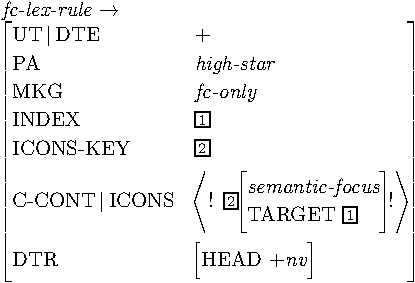
\includegraphics{pdf/fp-lex-rule.pdf}} \\ 
\evnup{b.} & \evnup{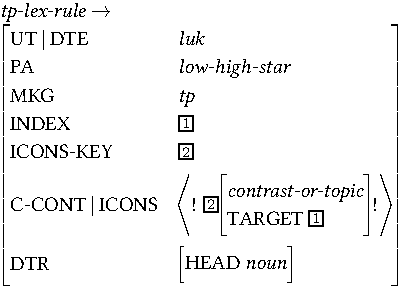
\includegraphics{pdf/tp-lex-rule.pdf}} \\
\end{tabular}}}






Building upon these rules, (\ref{exe:sample:derivation:eng}a) in which
\textit{\textsc{dog}} bears the A-accent for expressing
\tdl{semantic-focus} is constructed as
\myref{fig:the-dog-barks}.\is{MRS} The corresponding MRS and
dependency graph are presented in \myref{avm:the-dog-barks}.  The
utterance forms a clause, and the clausal type
(i.e.\ \tdl{declarative-clause} imposing [SF \tdl{prop-or-ques}]) is
inherited by the phrase structure type
(i.e.\ \tdl{head-subj-phrase}). Applying the constraint on
\tdl{clause} presented before, the CLAUSE-KEY of the NP \textit{the
  dog} points to the INDEX of the HEAD-DTR (i.e.\ the verb
\textit{barks}).\is{CLAUSE}\is{TARGET} The TARGET of the NP is
co-indexed with its INDEX, and the CLAUSE is co-indexed with the INDEX
of the verb. The TARGET and CLAUSE of \textit{barks} is recursively
linked. Each value in the \tdl{diff-list} of \isi{ICONS} is collected
into higher phrases.



\myexe{\enumsentence{\label{fig:the-dog-barks}
    \evnup{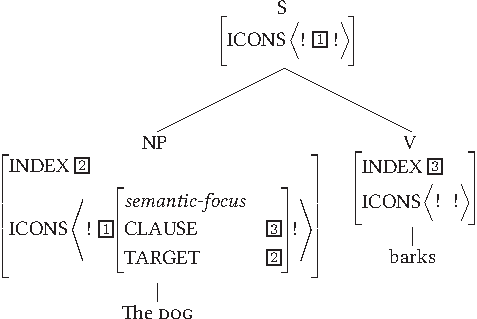
\includegraphics{pdf/the-dog-barks.pdf}}}}

\myexe{\eenumsentence{\toplabel{avm:the-dog-barks}
\item\evnup{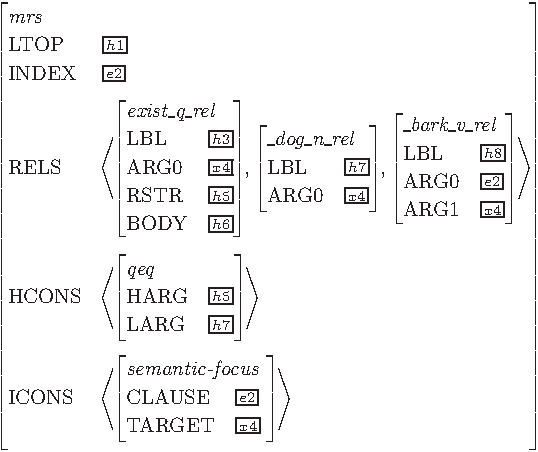
\includegraphics{pdf/emrs-the-dog-barks.pdf}}
\item\evnup{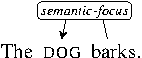
\includegraphics{pdf/basic1-eng.pdf}}}}


\subsection{Japanese and Korean}
\label{9:ssec:jpn:kor}


In \ili{Japanese} and \ili{Korean}, the distinction between lexical
markers (i.e.\ \ga \vs \wa in Japanese and \ika \vs \nun in Korean)
is responsible for delivering several different meanings with respect
to information structure. Note that case-marking NPs in \ili{Japanese} and
\ili{Korean} do not always correspond to A-accented NPs in
\ili{English}:\is{A-accent} NPs with \ga in Japanese or \ika in Korean
basically involve \tdl{non-topic}. On the other hand, A-accented NPs
in English are straightforwardly interpreted as possessing semantic
(i.e. non-contrastive) \isi{focus}.\is{non-contrastive focus}



\myexe{\enumsentence{\label{exe:sample:derivation:jpn}
\begin{tabular}[t]{llll}
a. & inu & ga & hoeru. \\
   & dog & \textsc{nom} & bark \\
b. & inu & wa & hoeru.\\
   & dog & \textsc{wa} & bark \\
   & \multicolumn{3}{l}{`The dog barks.' [jpn]} \\
\end{tabular}}}


\myexe{\enumsentence{\label{exe:sample:derivation:kor}
\begin{tabular}[t]{lll}
a. & kay-ka & cic-ta. \\
   & dog-\textsc{nom} & bark-\textsc{decl} \\
b. & kay-nun & cic-ta. \\
   & dog-\textsc{nun} & bark-\textsc{decl} \\
   & \multicolumn{2}{l}{`The dog barks.' [kor]} \\
\end{tabular}}}




In \ili{Japanese}, \ga and \wa are treated as adpositions,\is{adposition}
following the convention in \isi{Jacy} (\citealt{siegel:etal:16}).
The information structure value that the null marker assigns to
constituents is in line with \citet{yatabe:99}.  As for the null
marker \ensuremath{\emptyset}, the grammar developed here uses a lexical rule (in
\texttt{lrules.tdl} of the core of \lingo \isi{Grammar
  Matrix}).\footnote{This instance can be a daughter of a unary rule
  (i.e.\ \tdl{bare-np-phrase}) which promotes the word to a phrase.}
Although this is different from Yatabe's proposal (the null marking
system as particle ellipsis), I agree with \citeauthor{yatabe:99}'s
argument regarding the information structure meaning of null-marked
constituents in Japanese (and Korean). \citeauthor{yatabe:99} claims
that \ga cannot be dropped when the {\ga}-marked expression is
focused, which implies that null-marked phrases (mostly NPs) should be
evaluated as containing \tdl{non-focus}.  The AVMs for them are
provided in \myref{avm:ga:wa:jpn}.\is{ICONS-KEY} Note that the values
of MKG are not coreferenced with anything, and the element of
\isi{ICONS} specifies the relation of the complement, not of the
adposition itself.




\myexe{\enumsentence{\toplabel{avm:ga:wa:jpn}
\begin{tabular}[t]{ll}
\evnup{a.} & \evnup{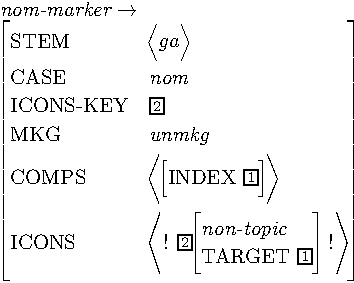
\includegraphics{pdf/nom-marker.pdf}} \\
\evnup{b.} & \evnup{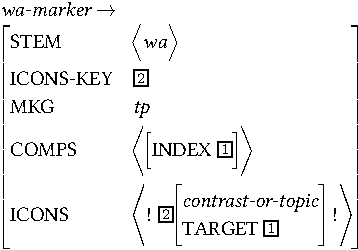
\includegraphics{pdf/top-marker.pdf}} \\
\evnup{c.} & \evnup{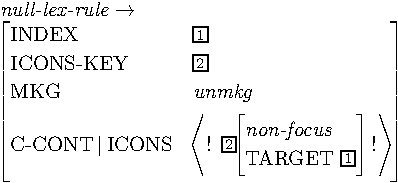
\includegraphics{pdf/null.pdf}} \\
\end{tabular}}}



The sample derivation for (\ref{exe:sample:derivation:jpn}a), in which
\textit{inu} `dog' is combined with \ga to indicate \tdl{non-topic},
is illustrated in \myref{fig:inu-ga-hoeru}.\footnote{In HPSG-based
  analyses for syntactic configuration in
  \ili{Japanese},\is{HPSG}\is{syntactic positioning} PPs are
  important.\is{syntactic positioning} That means the case markers
  (e.g.\ \ga for nominatives), the \wa marker, and a null-marker are
  adpositions that take the NPs that they are attached to as the
  complement, and constitute PPs.\is{adposition} The reason why the
  combination between NPs and the markers should be PPs in Japanese
  has been already explained in several previous HPSG-based studies
  \citep{gunji:87,siegel:99,yatabe:99}.}  The corresponding MRS
representation is given in (\ref{avm:inu-ga-hoeru}a),\is{MRS} and the
graphical version is in (\ref{avm:inu-ga-hoeru}b).



\myexe{\enumsentence{\label{fig:inu-ga-hoeru}
\evnup{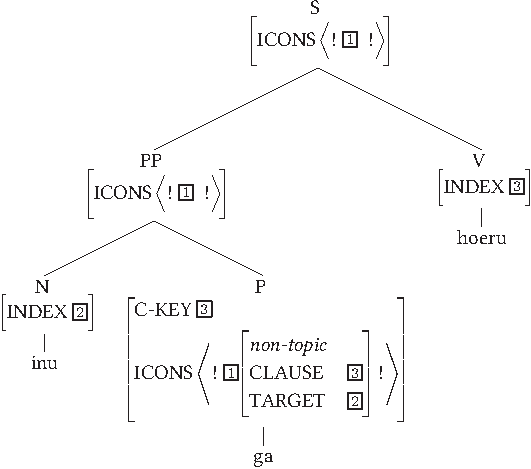
\includegraphics{pdf/inu-ga-hoeru.pdf}}}}


\myexe{\eenumsentence{\label{avm:inu-ga-hoeru}
\item\evnup{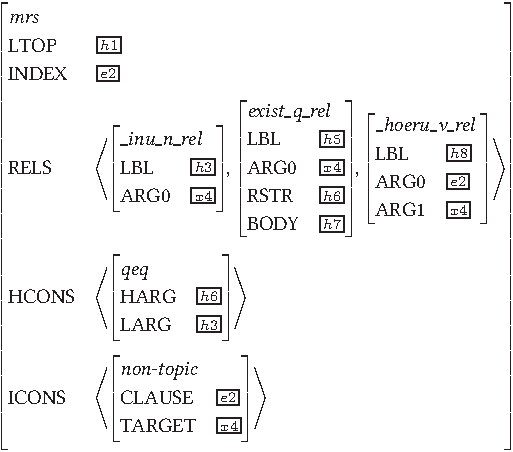
\includegraphics{pdf/jmrs.pdf}}
\item\evnup{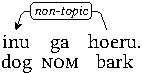
\includegraphics{pdf/basic1-jpn.pdf}}}}


\noindent The CLAUSE-KEY of the nominative marker \textit{ga} is
identified with its own
ICONS-KEY\ensuremath{\mid}CLAUSE.\is{ICONS-KEY}\is{CLAUSE-KEY} Second,
when the \tdl{head-comp-phrase} combines \textit{inu} and \textit{ga},
the ICONS-KEY\ensuremath{\mid}CLAUSE of \textit{inu} is identified
with the CLAUSE-KEY of \textit{ga}. The ICONS-KEY of \textit{ga} is
passed up to the mother (Semantic Inheritance
Principle).\footnote{``The CONTENT value of a phrase is
  token-identical to that of the head daughter.''
  \citep[48]{pollard:sag:94} } When the \tdl{head-subj-phrase}
combines \textit{inu ga} and \textit{hoeru}, the
ICONS-KEY\ensuremath{\mid}CLAUSE of the subject \textit{inu ga} is
identified with the INDEX of \textit{hoeru}.



With respect to \ili{Korean}, the present study basically assumes that
the marking systems (e.g.\ \wa or \onun-marking, case-marking, and
null-marking) in \ili{Japanese} and \ili{Korean} share the same
properties in terms of information structure, given that
counterexamples to this assumption are very rare.\footnote{One
  counterexample in which \wa and \nun show different behavior is
  reported in some Japanese dialects. For example, the Tokyo dialect
  does not show any difference from Korean with respect to using
  \isi{topic} markers, but the Kansai dialect sometimes makes a subtle
  difference in \wa-marking from \onun-marking in Korean.} Despite
similarity the resulting phrase structures in Korean have been
analyzed differently from those in Japanese. In a nutshell, \ga and
\wa in Japanese are dealt with as words, whereas \ika and \nun in
Korean are treated as suffixes.  Because postpositions are crucially
employed in the building blocks of a clause in most analyses of
Japanese syntax \citep{sato:tam:12}, the combination between nouns and
these markers (e.g.\ \ga, \wa, etc.)  forms a PP, rather than an
NP.\is{lexical markers} \citet{kim:yang:04}, in contrast, regard the
lexical markers in Korean (e.g.\ \ika, \nun, etc.) as affixes, rather
than adpositions.\footnote{Another approach to Korean postpositions is
  given in \citet{ko:08}, who insists that Korean postpositions should
  be analyzed as clitics attaching to either the preceding lexical
  item or weak syntactic heads sharing syntactic feature values of the
  complement phrase.}  That means that the combination between nouns
and their markers still remains as an NP. The present analysis
respects the two different analyses of these languages. Technically
speaking in the context of \isi{grammar engineering}, the adpositions
\ga and \wa in Japanese are treated as independent lexical entries,
while the morphemes \ika and \nun in Korean are dealt with by lexical
rules.  Accordingly, the derivation of an NP plus \ika or \nun is
created at the lexical level.  The inflectional rules are as follows.


\myexe{\enumsentence{\toplabel{avm:ika:nun:kor} 
\begin{tabular}[t]{ll}
\evnup{a.} & \evnup{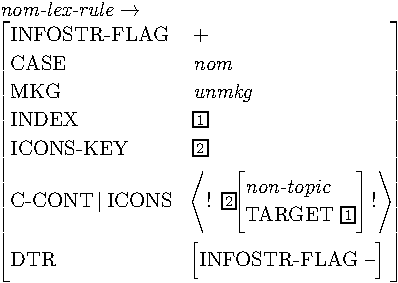
\includegraphics{pdf/ika.pdf}} \\
\evnup{b.} & \evnup{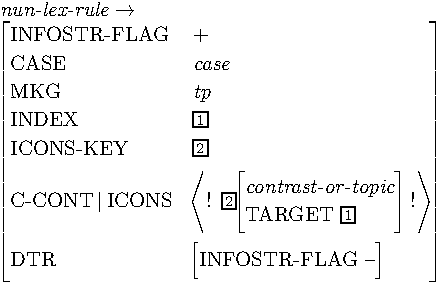
\includegraphics{pdf/nun.pdf}} \\
\evnup{c.} & \evnup{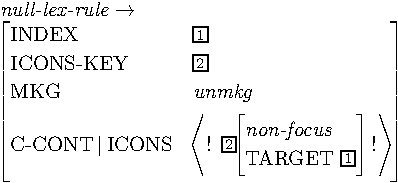
\includegraphics{pdf/null.pdf}} \\
\end{tabular}}}



\noindent Note that they are in complementary distribution. They share
the same slot in the morphological paradigm.  Additionally,
\tdl{null-lex-rule} is required to constrain information structure of
null-marked constituents.\footnote{Note, incidentally, that
  (\ref{avm:ika:nun:kor}c) for \ili{Korean} is the same as
  (\ref{avm:ga:wa:jpn}c) for \ili{Japanese}.}  Though the markers
represented in \myref{avm:ika:nun:kor} are realized as inflectional
rules in the morphological paradigm, the values of MKGs in Korean are
identical to those in Japanese,\is{MKG} and the elements on the ICONS
lists are the same as the values of COMPS{$\mid$}ICONS-KEY in
Japanese.\is{ICONS-KEY} Altogether, the analysis of Korean sentences
is syntactically similar to those in \ili{English}, and informatively
similar to those in Japanese. The sample derivation for
(\ref{exe:sample:derivation:kor}b), in which the \onun-marked
\textit{kay} `dog' is associated with \tdl{contrast-or-topic}, is
sketched out in (\ref{fig:kay-nun-cic-ta}a). The graphical
representation is also shown in (\ref{fig:kay-nun-cic-ta}b).

\myexe{\eenumsentence{\label{fig:kay-nun-cic-ta}
\item\evnup{\includegraphics{pdf/kay-nun-cic-ta.pdf}}
\item\evnup{\includegraphics{pdf/basic2-kor.pdf}}}}




\subsection{Russian}
\label{9:ssec:rus}


\ili{Russian} employs its relatively \isi{free word order} to mark
\isi{focus} with clause-final constituents bearing 
non-contrastive focus\is{non-contrastive focus} 
\citep{neeleman:titov:09}.\is{clause-final} Notably, constituents
in situ can also convey focus meaning, if they involve a
specific prosody for expressing focus.\is{prosody} Thus, in
(\ref{exe:sobaka:ch10-1}a) in the \isi{basic word order}, the focus
can fall on either the subject \textit{sobaka} or the verb
\textit{laet}, or both (i.e.\ \tdl{all-focus}). 
This is because Russian also employs prosody to signal focus.
This could be modeled by methods
similar to those we have use for \ili{English}.  Nonetheless, for ease of
explanation, we will limit our current focus to syntactic
position.\is{syntactic positioning}




\myexe{\enumsentence{\label{exe:sobaka:ch10-1}
\begin{tabular}[t]{lll}
a. & Sobaka & laet. \\
   & dog & bark \\
   & \multicolumn{2}{l}{`The dog barks.'} \\
b. & Laet & sobaka.\\
   & bark & dog \\
   & \multicolumn{2}{l}{`The \textsc{dog} barks.' [rus]} \\
\end{tabular}}}


Headed rules can have subtypes which handle information structure
differently, resolving the type of an \isi{ICONS} element or leaving
it underspecified.\is{underspecification} For example, the \ili{Russian} allosentences of
\myref{exe:sobaka:ch10-1} are instances of \tdl{head-subj-phrase}, but
the first one (\textit{sobaka laet}), in which the subject is
in situ, is licensed by a subtype that does not resolve the
\isi{ICONS} value, while the second one (\textit{laet
  sobaka}),\is{\textit{info-str}} in which the subject is marked
through being postposed, is licensed by a different one which
does. Hence, the subject \textit{in-situ} is specified as
\tdl{info-str} (i.e.\ underspecified), whereas the postposed subject
is specified as \tdl{focus}.  Consequently,
(\ref{exe:sobaka:ch10-1}a--b) are graphically represented as follows.



\myexe{\enumsentence{\toplabel{fig:basic:rus}
\begin{tabular}[t]{llll}
\evnup{a.} & \evnup{\includegraphics{pdf/basic2-rus.pdf}} & \evnup{b.} &
\evnup{\includegraphics{pdf/basic1-rus.pdf}} \\
\end{tabular}}}

In order to construct a derivation tree for (\ref{exe:sobaka:ch10-1}b)
whose word order is not neutral, it is necessary to implement several
additional devices: an additional flag feature [INFOSTR-FLAG
  \tdl{luk}], a unary phrase structure rule
\tdl{narrow-focused-phrase}, and \tdl{head-subj-phrase} (i.e.\ a
counterpart of the ordinary one
\tdl{subj-head-phrase}).\is{L-PERIPH}\is{R-PERIPH}\is{lightness}\is{narrow
  focus} First, the flag feature INFOSTR-FLAG is immediately under
SYNSEM like L/R-PERIPH and LIGHT.\footnote{Although they are housed in
  the same position, not all languages use INFOSTR-FLAG, while
  L/R-PERIPH and LIGHT are commonly used in human language. Thus, this
  flag feature is not included in the basic \tdl{synsem}.} This
feature serves to indicate whether the current phrase is information
structure-marked and includes an \isi{ICONS}
element. \tdl{Narrow-focused-phrase} takes only a constituent with
[INFOSTR-FLAG --] as its daughter, assigns [INFOSTR-FLAG +] to itself,
and introduces an \tdl{focus} element into the
C-CONT{$\mid$}ICONS.\footnote{Using C-CONT{$\mid$}ICONS for further
  constraining information structure values may raise one question.
  Given that ICONS is an accumulator list, like RELS and HCONS, some
  lexical rules and phrase structure rules that contribute a new
  \tdl{info-str} object can end up with more than one \tdl{info-str}
  object for the same CLAUSE/TARGET combination. This can be
  instantiated with Korean examples, although the rules are irrelevant
  to C-CONT.  In Korean, there are some lexical markers in Korean that
  participate in information structure; for example,
  \textit{kay-man-un} `dog-\textsc{only}-\textsc{nun}'. In this NP,
  \textit{man} adds one value into the ICONS list, and then
  \textit{un} adds another. This latent problem in the functionality
  of using the ICONS list needs to be resolved in further study.}
Finally, \tdl{head-subj-phrase} in \ili{Russian} inherits from both
\tdl{basic-head-subj-phrase} and \tdl{head-initial}. It takes a
constituent that has both [INFOSTR-FLAG +] and [R-PERIPH +] as its
non-head-daughter.  These indicate that the subject is marked for
information structure and that no constituent can be further attached
to the right. Recall that L-PERIPH and R-PERIPH are outside of
SYNSEM. Thus, the R-PERIPH value of \tdl{head-subj-phrase} is still
underspecified (i.e.\ \tdl{luk}), which allows the phrase to serve as
the head-daughter when combined with a peripheral frame-setter.


\tdl{Narrow-focused-phrase} and \tdl{head-subj-phrase} are represented
in the following AVMs.  The derivation tree for
(\ref{exe:sobaka:ch10-1}b) is sketched out in \myref{fig:laet-sobaka}.\is{narrow focus}


\myexe{\enumsentence{\toplabel{avm:rus:rule}
\begin{tabular}[t]{ll}
\evnup{a.} & \evnup{\includegraphics{pdf/narrow-focused-phrase.pdf}} \\
\evnup{b.} & \evnup{\includegraphics{pdf/head-subj-rule-rus.pdf}} \\
\end{tabular}}}


\myexe{\enumsentence{\label{fig:laet-sobaka}
\evnup{\includegraphics{pdf/laet-sobaka.pdf}}}}


\section{Summary}
\label{10-1:sec:summary}

This chapter has discussed specifics of implementing \isi{ICONS} into
lexical and phrasal types for constraining information
structure. Lexical types inherit from one of four potential types of
\tdl{icons-lex-item}: \tdl{no-icons-lex-item},
\tdl{basic-icons-lex-item}, \tdl{one-icons-lex-item}, and
\tdl{two-icons-lex-item}.  Both \tdl{no-icons-lex-item} and
\tdl{basic-icons-lex-item} have an empty \isi{ICONS} list, and
\tdl{no-icons-lex-item} is additionally [MKG [FC \tdl{na}, TP
    \tdl{na}]].\is{MKG} This constraint indicates that lexical entries
which inherit from \tdl{no-icons-lex-item} cannot be marked with
respect to information structure; for instance, relative pronouns,
expletives, etc.  Nominal items normally inherit from
\tdl{basic-icons-lex-item}, while inheritance for verbal items is
determined by how many clauses are subordinated to the verbal
item.\is{adposition} Adpositions and determiners inherit from either
\tdl{basic-icons-lex-item} or \tdl{one-icons-lex-item}, adverbs
inherit from \tdl{basic-icons-lex-item}, and syncategorematic items
inherit from \tdl{no-icons-lex-item}. Conjunctions may or may not
introduce a \tdl{topic} value into \isi{ICONS} depending on which type
of adverbial clauses they involve. The values of CLAUSE are identified
when \tdl{basic-head-subj-phrase} is constructed.\is{CLAUSE}
\tdl{Basic-head-mod-phrase-simple} and \tdl{head-filler-phrase} have
some extra constraints to specify which element is linked to which
clause.\is{clause-initial}\is{clause-final} There are three additional
constraints for elaborating on properties of information structure:
L/R-PERIPH, LIGHT, and PHON.  L/R-PERIPH constrain the
clause-initial/final positioning of constituents, and likewise LIGHT
is used for constraining \isi{preverbal} and \isi{postverbal}
constituents. PHON is included in \texttt{matrix.tdl} of the core of
\lingo \isi{Grammar Matrix} for use in future work with acoustic
resolution systems.

